\section{Consequences}\label{sec:consequences}

Throughout this section the axioms of Theorem~\ref{thm:A} and the labelling convention \ax{S} hold, $\LR=\bracket{I_h}{I_g}$, and for
$\beta\neq1$ we put
\[
 \rho_\beta:=\frac{\rho-\beta\Pi}{1-\beta},\qquad
 k_\beta:=\frac{h-\beta g}{1-\beta}=g+\frac{h-g}{1-\beta}\in\Hset_1 .
\]

\begin{corollary}[Association]\label{cor:assoc}
\begin{enumerate}[label=(\alph*),nosep]
\item $\rho_\beta=I_{k_\beta}$ is cash additive of slope $1$, and $\rho_\beta(X)=0\iff\LR(X)\in\{\beta,\star\}$.
  Hence $\LR(X)=\beta\iff\rho_\beta(X)=0$ holds exactly off $\{\rho=\Pi=0\}=\{\LR=\star\}$; it fails, for instance, at
  $X=0$ and at $X-\rho(X)$ for every $X\in N$.
\item For $X\notin N$: $\LR(X-m)=\beta\iff m=\rho_\beta(X)$, and then $\Pi(X)-m=(\Pi(X)-\rho(X))/(1-\beta)\ne0$.
\item For $X\in N$: $\LR(X-m)\in\{1,\star\}$ for every $m$.
\item $\rho_\beta$ is $\TV(k_\beta)$-Lipschitz; in Theorem~\ref{thm:B}, $\TV(k_\beta)\le(1+|\beta|)/|1-\beta|$.
\item $\rho_\beta$ is monotone iff $k_\beta$ is non-decreasing. If $h\ne g$, $\rho_\beta$ is \emph{not} monotone for
  all $\beta$ in a punctured neighbourhood of $1$.
\end{enumerate}
\end{corollary}

\begin{proof}
(a) $\rho_\beta(X)=0\iff\rho(X)=\beta\Pi(X)$; if $\Pi(X)\ne0$ this says $\LR(X)=\beta$, and if $\Pi(X)=0$ it says
$\rho(X)=0$, i.e.\ $\LR(X)=\star$. Conversely $\LR(X)=\star$ means $\rho=\Pi=0$. At $X\in N$, $Y=X-\rho(X)$ has
$\rho(Y)=\Pi(Y)=0$, so $\LR(Y)=\star\ne\beta$ while $\rho_\beta(Y)=0$.
(b) $\LR(X-m)=\beta\iff\rho-m=\beta(\Pi-m)\iff m=\rho_\beta(X)$, and
$\Pi-\rho_\beta=(\Pi-\rho)/(1-\beta)\neq0$ off $N$.
(c) On $N$ the cash line equals $1$ away from its price point (Proposition~\ref{prop:readings}(d)).
(d) Lemma~\ref{lem:cashlip} and the Lipschitz bound for $I_{k}$.
(e) $I_{k}$ is monotone iff $k$ is non-decreasing. Since $h-g$ vanishes at $0$ and $1$ and is non-constant, there are
$p<q$ with $(h-g)(p)>(h-g)(q)$ and $p'<q'$ with $(h-g)(p')<(h-g)(q')$. As $\beta\to1$,
$(1-\beta)k_\beta=h-\beta g\to h-g$ uniformly, so for $\beta$ near $1$ both strict inequalities persist for
$k_\beta$, whatever the sign of $1-\beta$. \qedhere
\end{proof}

Part (e) is the counterpart of Proposition~\ref{prop:F2} for the associated family: even when $\rho$ and $\Pi$ are
distortion premia, $\rho_\beta$ is in general a signed Choquet integral.

\begin{example}\label{ex:family}
Let $h=\mathrm{id}$ and $g=\sqrt{\cdot}$. Then $k_\beta(p)=(p-\beta\sqrt p)/(1-\beta)$ and
$k_\beta'(p)=\big(1-\beta/(2\sqrt p)\big)/(1-\beta)$. For $\beta<1$, $k_\beta$ is non-decreasing if and only if
$\beta\le2\sqrt p$ for all $p\in(0,1]$, that is, $\beta\le0$; for $\beta>1$ it is non-decreasing if and only if
$\beta\ge2\sqrt p$ for all $p$, that is, $\beta\ge2$. Hence $\rho_\beta$ is a distortion premium if and only if
$\beta\notin(0,2)$; for $\beta\in(0,1)\cup(1,2)$ it is a signed Choquet integral that is not monotone
(Figure~\ref{fig:family}).
\end{example}

\begin{figure}[ht]
\centering
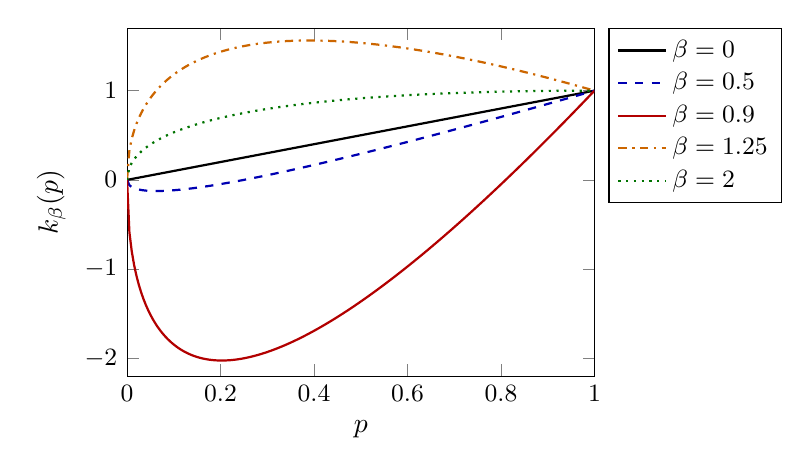
\begin{tikzpicture}
\begin{axis}[width=0.62\textwidth,height=6cm,xmin=0,xmax=1,ymin=-2.2,ymax=1.7,
  xlabel={$p$},ylabel={$k_\beta(p)$},tick label style={font=\small},samples=200,domain=0:1,
  legend pos=outer north east,legend style={font=\small,cells={anchor=west}}]
\addplot[thick,black] {x}; \addlegendentry{$\beta=0$}
\addplot[thick,blue!70!black,dashed] {(x-0.5*sqrt(x))/0.5}; \addlegendentry{$\beta=0.5$}
\addplot[thick,red!70!black] {(x-0.9*sqrt(x))/0.1}; \addlegendentry{$\beta=0.9$}
\addplot[thick,orange!80!black,dashdotted] {(x-1.25*sqrt(x))/(-0.25)}; \addlegendentry{$\beta=1.25$}
\addplot[thick,green!45!black,dotted] {(x-2*sqrt(x))/(-1)}; \addlegendentry{$\beta=2$}
\end{axis}
\end{tikzpicture}
\caption{The distortions $k_\beta$ of the associated family in Example~\ref{ex:family} ($h=\mathrm{id}$,
$g=\sqrt{\cdot}$). They are monotone for $\beta=0$ and $\beta=2$ and not monotone for $\beta\in(0,1)\cup(1,2)$.}
\label{fig:family}
\end{figure}

\begin{corollary}[Pooling at non-finite values]\label{cor:projpool}
Assume the axioms of Theorem~\ref{thm:A} and \ax{S}. Then for all comonotone $X,Y$,
\[
 \LR(X+Y)=\bracket{\rho(X)+\rho(Y)}{\Pi(X)+\Pi(Y)} .
\]
In terms of loss ratios and implied premiums alone:
\begin{center}\small
\begin{tabularx}{0.95\textwidth}{@{}>{\raggedright\arraybackslash}p{5.4cm}>{\raggedright\arraybackslash}X@{}}
\toprule
\textbf{Case} & \textbf{Pooled loss ratio}\\
\midrule
$X,Y\in D$, $\Pi(X)+\Pi(Y)\ne0$ & premium-weighted mean (\axCM)\\
$X,Y\in D$, premiums cancel & $\infty$ if $\LR(X)\ne\LR(Y)$; $\star$ if $\LR(X)=\LR(Y)$\\
$\Pi(X)=0$, $Y\in D$ & $\LR(Y)+\rho(X)/\Pi(Y)$, with $\rho(X)=\lim_{c\to0}c\,\LR(X+c)$\\
$\Pi(X)=\Pi(Y)=0$ & $\infty$ unless $\rho(X)=-\rho(Y)$, in which case $\star$\\
\bottomrule
\end{tabularx}
\end{center}
\end{corollary}

\begin{proof}
$\rho$ and $\Pi$ are comonotonic additive (Lemma~\ref{lem:comon}) and $\LR=\bracket{\rho}{\Pi}$ under \ax{S}
(Theorem~\ref{thm:A}). The table spells out $\bracket{\rho(X)+\rho(Y)}{\Pi(X)+\Pi(Y)}$, using $\rho=\Pi\,\LR$ on $D$
and Proposition~\ref{prop:readings}(c) for books with zero premium. If premiums cancel,
$\rho(X)+\rho(Y)=\Pi(X)(\LR(X)-\LR(Y))$. \qedhere
\end{proof}

The third row has a direct reading: a loss that is carried without premium adds its size, relative to the
premium base, to the loss ratio of the book it joins.

\begin{corollary}[Orderings, convexity and shape within the class]\label{cor:shape}
\begin{enumerate}[label=(\alph*)]
\item \emph{Endpoints.} $\rho$ is monotone iff $h$ is non-decreasing; $\rho$ is convex iff $h$ is concave
  \citep[Thm.~3]{www2020}; $\rho$ is coherent iff $h$ is concave and non-decreasing, in which case $\rho$ is a
  mixture of expected shortfalls $\mathrm{ES}_\alpha$ over levels $\alpha\in[0,1]$, with the convention
  $\mathrm{ES}_1:=\operatorname{ess\,sup}$ \citep{kusuoka2001,jst2006,folmerschied2016} and \citet[Thm.~5]{www2020b}; the endpoint is needed, for
  instance, for $h=\1_{(0,1]}$, which gives $\rho=\operatorname{ess\,sup}$. The same holds for $\Pi$ and $g$.
\item \emph{Ordering.} $\LR\le1$ on $\{\Pi>0\}$ iff $h\le g$.
\item \emph{Convex acceptance cones.} For $\beta\ne1$ let $A_\beta:=\{\rho\le\beta\Pi\}=\{I_{h-\beta g}\le0\}$.
  Then $A_\beta$ is convex iff $h-\beta g$ is concave, and all $A_\beta$, $\beta\in[0,\infty)\setminus\{1\}$, are
  convex iff $h$ is concave and $g$ is convex.
\item \emph{Quasi-convexity and quasi-concavity (sufficient conditions).}
  If $h$ is concave and $g$ is convex, then $\{\Pi>0\}$ is convex, $\LR\ge1$ there, and $\LR$ is quasi-convex on it.
  If, in Theorem~\ref{thm:B} with $g>0$, $h$ is convex and $g$ is concave, then $\LR\le1$ on $\Xp$ and $\LR$ is
  quasi-concave on $\Xp$. In particular the actuarial ratio $\E/C_g$ with $g$ concave is quasi-\emph{concave}.
\item \emph{Rigidity.} $\rho_\beta$ is convex for all $\beta\in[0,\infty)\setminus\{1\}$ iff $h=g$ and $g$ is concave.
\end{enumerate}
\end{corollary}

\begin{proof}
(a) The monotonicity criterion is in \citet{www2020}, see also \citet[Prop.~2]{www2020b}, and the
convexity criterion is \citet[Thm.~3]{www2020}.
(b) If $h\le g$ then $g-h\ge0$ with $(g-h)(1)=0$, so $I_{g-h}\ge0$ and $\LR\le1$ where $\Pi>0$. If $h(p)>g(p)$ for some $p$,
then $\LR(\1_A+c)=(h(p)+c)/(g(p)+c)>1$ for large $c$, where the premium $g(p)+c$ is positive.
(c) $I_{h-\beta g}$ has cash slope $1-\beta\ne0$, so all its sublevel sets are translates of $A_\beta$; hence
convexity of $A_\beta$ is quasi-convexity of $I_{h-\beta g}$, which is equivalent to concavity of $h-\beta g$
\citep[Thm.~3]{www2020}. Taking $\beta=0$ and $\beta\to\infty$ in $(h-\beta g)/\beta$ gives the second statement.
(d) If $h$ is concave and $g$ is convex then $I_g$ is concave, so $\{I_g>0\}$ is convex; $h\ge\mathrm{id}\ge g$, so
$\LR\ge1$; and for $\beta\ge1$ the set $\{I_h-\beta I_g\le0\}$ is convex because $h-\beta g$ is concave. If
$h$ is convex and $g$ concave, then $h\le\mathrm{id}\le g$, and $I_h-tI_g$ is concave for $t\ge0$, so
$\{\LR\ge t\}$ is convex; for $t<0$ the superlevel set is all of $\Xp$, since $I_h\ge0$ and $I_g>0$ on $\Xp$.
(e) Convexity of $\rho_\beta=I_{k_\beta}$ for $\beta<1$ means $h-\beta g$ concave, and for $\beta>1$ means
$h-\beta g$ convex. Letting $\beta\to1^\mp$ gives $h-g$ concave and convex, hence affine with zero endpoints, i.e.\
$h=g$; then $k_\beta=g$ and $\rho_\beta$ is convex iff $g$ is concave. The converse is clear. \qedhere
\end{proof}

In particular, the actuarial ratio $\E/C_g$ with $g$ concave is quasi-concave and not, in general, quasi-convex.

\begin{example}\label{ex:qc}
Let $A,B$ be disjoint with $P(A)=0.2$, $P(B)=0.3$, and $X_t=(1-t)\1_A+t\1_B$, $t\in[0,1]$. For
$\mathrm{ES}_{0.9}/\E$ (Example~\ref{ex:ES}), $\mathrm{ES}_{0.9}(X_t)=\max\{1-t,t\}$ and
$\LR(X_t)=\max\{1-t,t\}/(0.2+0.1t)$, which equals $5$ at $t=0$, $10/3$ at $t=1$ and $2$ at $t=\tfrac12$: the ratio
lies below the larger endpoint value, as quasi-convexity requires. For $\E/C_{\sqrt{\cdot}}$ the ratio equals
$\sqrt{0.2}\approx0.447$ at $t=0$, $\sqrt{0.3}\approx0.548$ at $t=1$ and $\sqrt{0.5}\approx0.707$ at $t=\tfrac12$: it lies
above the smaller endpoint value, as quasi-concavity requires (Figure~\ref{fig:qc}).
\end{example}

\begin{figure}[ht]
\centering
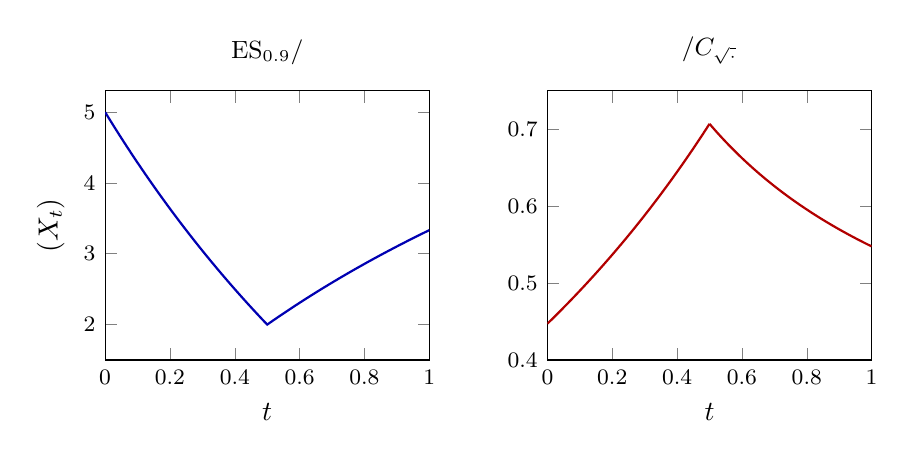
\begin{tikzpicture}
\begin{axis}[name=l,width=0.47\textwidth,height=5cm,xmin=0,xmax=1,ymin=1.5,ymax=5.3,xlabel={$t$},
  ylabel={$\LR(X_t)$},title={\small $\mathrm{ES}_{0.9}/\E$},tick label style={font=\footnotesize},samples=101,domain=0:1]
\addplot[thick,blue!70!black] {max(1-x,x)/(0.2+0.1*x)};
\end{axis}
\begin{axis}[at={(l.south east)},xshift=1.5cm,width=0.47\textwidth,height=5cm,xmin=0,xmax=1,ymin=0.4,ymax=0.75,
  xlabel={$t$},title={\small $\E/C_{\sqrt{\cdot}}$},tick label style={font=\footnotesize},samples=60]
\addplot[thick,red!70!black,domain=0:0.5] {(0.2+0.1*x)/(0.70711*x+0.44721*(1-2*x))};
\addplot[thick,red!70!black,domain=0.5:1] {(0.2+0.1*x)/(0.70711*(1-x)+0.54772*(2*x-1))};
\end{axis}
\end{tikzpicture}
\caption{Loss ratios along the segment $X_t=(1-t)\1_A+t\1_B$ of Example~\ref{ex:qc}: quasi-convex for
$\mathrm{ES}_{0.9}/\E$ (left) and quasi-concave for $\E/C_{\sqrt{\cdot}}$ (right).}\label{fig:qc}
\end{figure}

\begin{example}[Further special cases]
(1) \emph{Wang--Young--Panjer pairs} on nonnegative losses: Theorem~\ref{thm:C}.
(2) \emph{Coherent pairs}: $h,g$ concave non-decreasing; $\rho_\beta$ is a signed mixture of expected shortfalls.
(3) \emph{Actuarial ratio} $\E/C_g$, $h=\mathrm{id}$: Proposition~\ref{prop:unique} gives $g(p)=p/\LR(\1_A)$ for $P(A)=p$, so the
premium distortion is identified from the loss ratios of Bernoulli books.
(4) \emph{VaR-type pairs} are admissible in Theorem~\ref{thm:B}; $\rho_\beta$ is non-monotone near $\beta=1$; a
VaR-type premium $g=\1_{(a,1]}$ is excluded from Theorem~\ref{thm:C}, since $g>0$ fails.
(5) \emph{Gini-type ratios}: $\LR-1=I_{h-g}/I_g$ is a location-invariant signed Choquet ``variability'' divided by a
premium (compare \citealp{bfww2022}).
\end{example}
